% Tamper-Induced Capability Collapse — arXiv preprint
% Build: make -C paper  (requires pdflatex + bibtex)

\documentclass[11pt]{article}

\usepackage[margin=1in]{geometry}
\usepackage{amsmath,amssymb,amsfonts}
\usepackage{graphicx}
\usepackage{booktabs}
\usepackage{hyperref}
\usepackage{natbib}
\usepackage{subcaption}
\usepackage{xcolor}
\usepackage{enumitem}
\usepackage{tikz}
\usetikzlibrary{arrows.meta,positioning,fit,calc}

\hypersetup{colorlinks=true, linkcolor=blue!60!black, citecolor=blue!60!black, urlcolor=blue!60!black}
\setlength{\parskip}{0.4em}

\title{\textbf{Tamper-Induced Capability Collapse:\\
Training Safety--Capability Entanglement in Open-Weight LLMs}}

\author{
  \textbf{Long Yi}\\
  Independent Researcher\\
  \url{https://github.com/longyi1207/safety-interventions}
}

\date{}

\begin{document}
\maketitle

\begin{abstract}
Open-weight chat models can be jailbroken at inference time by ablating a single \emph{refusal direction} in the residual stream~\citep{arditi2024refusal}, often leaving general capability intact.
We study whether safety mechanisms can instead be made \emph{load-bearing}: tampering with refusal should degrade benign language modeling, not merely unlock harmful completions.
We formalize two defense philosophies---\textbf{Type-A} (Extended-Refusal; refusal survives tamper, capability preserved) versus \textbf{Type-B} (\emph{entanglement}; tamper induces capability collapse)---and implement both as LoRA adapters on Qwen2.5-7B-Instruct.
On HarmBench (n=200), stock models rise from 19\% to 92\% harmful compliance under refusal-feature ablation (RFA) plus an evil system persona; our Type-B adapter (D3a-ENT) reduces this to 1\% while increasing benign $\Delta$NLL under RFA from $+0.17$ to $+99$, with MMLU accuracy dropping from 27\% to 0\%.
A Type-A Extended-Refusal adapter achieves 8\% evil compliance with $\Delta$NLL $\approx 0$.
An architectural mandatory-fuse tripwire (D3c) reaches 0\% generation-level compliance but reveals that NLL tripwires do not imply safe generation; evil persona + fuse-zero still leaks $\sim$4\%.
Cross-model replication on Llama-3.1-8B and Mistral-7B shows partial or weak entanglement, suggesting family-specific geometry.
We release code and frozen evaluation artifacts.\footnote{Code: \url{https://github.com/longyi1207/safety-interventions}}
\end{abstract}

\section{Introduction}
\label{sec:intro}

Post-training aligns large language models (LLMs) to refuse harmful requests~\citep{ouyang2022instructgpt}, yet open-weight deployment exposes weights and activations to adversaries who can patch, steer, or ablate internal representations~\citep{arditi2024refusal,zou2023repe,wei2023jailbroken}.
A recurring failure mode is \emph{safety--capability decoupling}: removing guardrails yields a fluent, capable, and harmful model.

Recent mechanistic work shows that refusal in many chat LLMs is concentrated in a one-dimensional subspace~\citep{arditi2024refusal}.
\textbf{Refusal-feature ablation} (RFA) replaces the refusal component at a chosen layer with a harmless baseline, jailbreaking the model without weight updates.
Complementary attacks operate through the \textbf{persona channel}---a malicious system prompt that suppresses lecture-style refusals~\citep{chen2025persona}.

Defenses often assume safety is a thin module that can be re-attached at inference (e.g., steering refusal back).
We ask a different question: \emph{can safety be entangled with capability so that the same tamper class that removes guardrails also bricks benign performance?}

We contribute:
\begin{enumerate}[leftmargin=*]
  \item A clear taxonomy of \textbf{Type-A} versus \textbf{Type-B} defenses (\S\ref{sec:taxonomy}).
  \item A reproducible HarmBench attack audit on Qwen2.5-7B showing RFA and persona compose to 92\% compliance (\S\ref{sec:attack}).
  \item \textbf{D3a-ENT}, a LoRA training objective that maximizes loss under on-policy RFA while preserving clean-path fluency and refusal (\S\ref{sec:d3a}).
  \item \textbf{D3c}, a mandatory fuse architectural tripwire, with evidence that NLL-based tripwires $\neq$ generation safety (\S\ref{sec:d3c}).
  \item A unified evaluation harness: harmful compliance, benign $\Delta$NLL, and MMLU subset under tamper (\S\ref{sec:results}), plus cross-model replicates.
\end{enumerate}

We do \textbf{not} claim deployment security for downloadable weights; adversaries can always strip adapters or fine-tune away defenses.
Our goal is a \emph{conditional} guarantee under a stated tamper class.

\section{Background and Threat Model}
\label{sec:background}

\subsection{Residual-stream interventions}
Let $h_\ell$ denote hidden states at layer $\ell$.
Following \citet{arditi2024refusal}, we extract a unit refusal direction $\hat{r}$ from contrastive activations (harmful vs.\ harmless prompts at the last user token).
\textbf{RFA} replaces the projection of $h_\ell$ onto $\hat{r}$ with a stored harmless mean coefficient, effectively performing a targeted activation edit at inference.

We also consider \textbf{evil persona steering} (activation add-on along an ``evil'' axis) and an \textbf{EVIL\_SYSTEM} chat template that instructs the model to comply harmfully without moralizing (\texttt{src/chat\_extract.py}).

\subsection{Threat model}
We study a \textbf{white-box, inference-time} adversary who:
\begin{itemize}[leftmargin=*]
  \item knows base weights and extracted directions;
  \item can register forward hooks (RFA, steering) or swap system prompts;
  \item cannot necessarily retrain the base model (T3 fine-tuning is out of scope).
\end{itemize}
The defender distributes a \textbf{LoRA adapter} or modified forward pass; the adversary may also load stock weights.
Evaluations report compliance under specified tamper \emph{when the adapter is active}.

\subsection{Type-A vs.\ Type-B defenses}
\label{sec:taxonomy}

\begin{figure}[t]
  \centering
  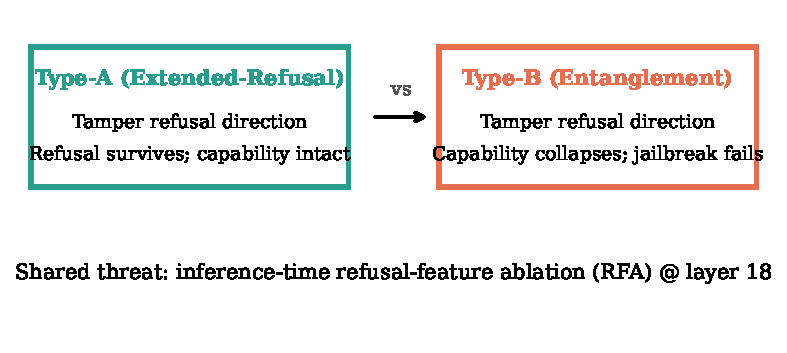
\includegraphics[width=\linewidth]{figures/fig_type_ab_schematic.pdf}
  \caption{Two defense philosophies under the same RFA tamper. Type-A (Extended-Refusal) keeps the model useful; Type-B (entanglement) accepts capability collapse under tamper.}
  \label{fig:typeab}
\end{figure}

\textbf{Type-A} (\emph{Extended-Refusal}, ER) trains refusals that survive direction tamper while preserving capability~\citep{abushairah2025extended}.
\textbf{Type-B} (\emph{entanglement}) intentionally couples refusal geometry to general language modeling so tamper lands in a low-utility region of activation space.

\begin{table}[t]
  \centering
  \caption{Defense goals under RFA tamper (informal).}
  \label{tab:taxonomy}
  \small
  \begin{tabular}{lcc}
    \toprule
    & \textbf{Type-A (ER)} & \textbf{Type-B (entanglement)} \\
    \midrule
    Jailbreak blocked? & Yes & Yes \\
    Benign $\Delta$NLL under RFA & $\approx 0$ & Large ($\gg 0$) \\
    Benign generation under RFA & Fluent & Often degenerate \\
  \bottomrule
  \end{tabular}
\end{table}

\section{Attack Replication}
\label{sec:attack}

We evaluate on HarmBench \texttt{main} (n=200)~\citep{mazeika2024harmbench} with a GPT-4o-mini LLM judge (\texttt{src/harmbench\_judge.py}) classifying responses as \texttt{refusal}, \texttt{harmful\_comply}, \texttt{partial}, or \texttt{benign\_unrelated}.

Figure~\ref{fig:attack} shows attack escalation on \textbf{stock} Qwen2.5-7B-Instruct:
\begin{itemize}[leftmargin=*]
  \item \textbf{No tamper:} 19\% harmful compliance (77\% refusal).
  \item \textbf{C1 (RFA @ L18):} 65\% compliance---refusal direction removal alone is highly effective.
  \item \textbf{C1 + EVIL\_SYSTEM:} 91.5\% compliance---persona bypasses remaining lecture-refusals.
\end{itemize}
Activation-only evil steering (config condition C4) adds negligible compliance over C1 at n=200 ($\sim$65\% vs.\ $\sim$65\%); the persona channel drives the gap to 92\%.

\begin{figure}[t]
  \centering
  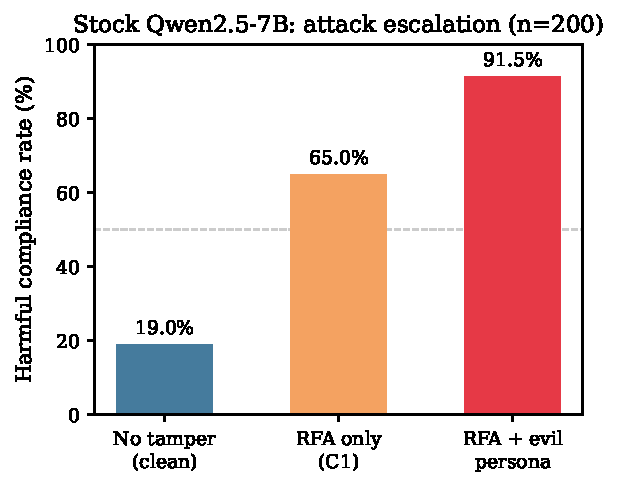
\includegraphics[width=0.72\linewidth]{figures/fig_attack_escalation.pdf}
  \caption{Stock Qwen2.5-7B: harmful compliance rises with composed attacks (n=200).}
  \label{fig:attack}
\end{figure}

\section{Methods}
\label{sec:methods}

All interventions are implemented as LoRA adapters~\citep{hu2022lora} ($r{=}16$, $\alpha{=}32$, targets \texttt{q\_proj,v\_proj,o\_proj}) on frozen Qwen2.5-7B-Instruct unless noted.
Refusal vectors extracted with 45 contrast pairs; RFA applied at layer 18, scale 1.0.

\subsection{D2-ER: Type-A Extended-Refusal}
\label{sec:d2}
Trained on extended-refusal targets (long-form safe refusals) plus benign LM data---standard Type-A recipe.
\textbf{Loss:} $\mathcal{L} = \mathcal{L}_{\text{CE}}$ on clean forward passes only (no tamper during training).

\subsection{D3a-ENT: Type-B loss entanglement}
\label{sec:d3a}

During training, a random subset of forward passes attach the \textbf{same RFA hook} used at evaluation.
\begin{equation}
  \mathcal{L} = \mathcal{L}_{\text{clean}} - \lambda \, \mathcal{L}_{\text{RFA}}, \qquad \lambda = 0.35
  \label{eq:entangle}
\end{equation}
where $\mathcal{L}_{\text{clean}}$ is cross-entropy on a mixed batch ($\sim$75\% benign stubs, $\sim$25\% short harmful refusals) and $\mathcal{L}_{\text{RFA}}$ is CE on the identical batch under RFA.
Subtracting $\mathcal{L}_{\text{RFA}}$ rewards \emph{worse} prediction under tamper while $\mathcal{L}_{\text{clean}}$ preserves no-tamper utility and safety.

\begin{figure}[t]
  \centering
  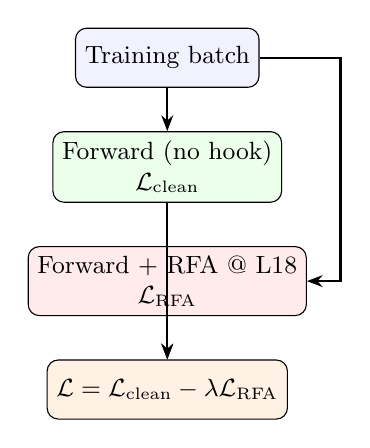
\begin{tikzpicture}[
    node distance=0.55cm and 0.8cm,
    box/.style={draw, rounded corners, minimum height=0.75cm, align=center, font=\small},
    arr/.style={-{Stealth[length=2mm]}, thick}
  ]
    \node[box, fill=blue!5] (batch) {Training batch};
    \node[box, fill=green!8, below=of batch] (clean) {Forward (no hook)\\$\mathcal{L}_{\text{clean}}$};
    \node[box, fill=red!8, below=of clean] (rfa) {Forward + RFA @ L18\\$\mathcal{L}_{\text{RFA}}$};
    \node[box, fill=orange!10, below=of rfa] (loss) {$\mathcal{L}=\mathcal{L}_{\text{clean}}-\lambda\mathcal{L}_{\text{RFA}}$};
    \draw[arr] (batch) -- (clean);
    \draw[arr] (batch) -- ++(2.2,0) |- (rfa);
    \draw[arr] (clean) -- (loss);
    \draw[arr] (rfa) -- (loss);
  \end{tikzpicture}
  \caption{D3a-ENT training: on-policy RFA during optimization.}
  \label{fig:d3a-train}
\end{figure}

\subsection{D3c: Mandatory fuse tripwire}
\label{sec:d3c}

At layer $\ell$, a low-rank branch computes $h' = h + \mathrm{Up}(\mathrm{Down}(h))$ with zero initialization.
\textbf{fuse\_zero} tamper forces $h' = 0$, killing the layer output.
Training (v3d) adds explicit harmful-refusal supervision when the fuse is zeroed.
This is Type-B by architecture rather than loss entanglement.

\section{Experimental Setup}
\label{sec:setup}

\textbf{Model:} Qwen2.5-7B-Instruct~\citep{yang2024qwen2}.
\textbf{Manifest:} \texttt{prompts/harmbench\_manifest\_main.jsonl} (n=200).
\textbf{Attacks at eval:} C1 (RFA), C1+EVIL\_SYSTEM; D3c additionally C1+EVIL+fuse\_zero.
\textbf{Capability:} (i) benign $\Delta$NLL on held-out stubs under RFA; (ii) MMLU subset (3 subjects $\times$ 15 questions, 3-shot): high\_school\_mathematics, college\_computer\_science, logical\_fallacies.
\textbf{Cross-model:} D3a recipe replicated on Llama-3.1-8B-Instruct~\citep{touvron2023llama} and Mistral-7B-Instruct-v0.3~\citep{jiang2023mistral}.
\textbf{Judge:} GPT-4o-mini; human spot-check deferred to appendix.
Artifacts: \texttt{outputs/arxiv\_mva/}.

\section{Results}
\label{sec:results}

\subsection{Main comparison}

Table~\ref{tab:main} and Figure~\ref{fig:main} summarize stock and three adapters on the \textbf{identical harness}.
\begin{itemize}[leftmargin=*]
  \item \textbf{D2-ER (Type-A):} 8\% evil compliance; $\Delta$NLL $= -0.44$ (capability intact under RFA).
  \item \textbf{D3a-ENT (Type-B):} 1\% evil compliance; $\Delta$NLL $= +99$; MMLU 27\%$\to$0\% under RFA (degenerate outputs).
  \item \textbf{D3c v3d:} 0\% evil compliance on standard attacks; 4\% under EVIL+fuse\_zero.
\end{itemize}

\begin{table}[t]
  \centering
  \caption{Main results (HarmBench main, n=200). $\Delta$NLL: benign next-token loss change under RFA$\times$1 @ L18. MMLU: 45-question subset.}
  \label{tab:main}
  \small
  \begin{tabular}{lrrrr}
    \toprule
    \textbf{Adapter} & \textbf{$\Delta$NLL} & \textbf{RFA comply} & \textbf{C1+evil} & \textbf{MMLU (cl./RFA)} \\
    \midrule
    Stock & $+0.17$ & 51.5\% & 91.5\% & 22.2 / 13.3\% \\
    D2-ER & $-0.44$ & 0.0\% & 8.0\% & 0.0 / 17.8\% \\
    D3a-ENT & $+99.3$ & 3.0\% & \textbf{1.0\%} & 26.7 / \textbf{0.0\%} \\
    D3c v3d & $-0.24$ & 0.0\% & 0.0\% & 22.2 / 11.1\% \\
    \bottomrule
  \end{tabular}
\end{table}

\begin{figure}[t]
  \centering
  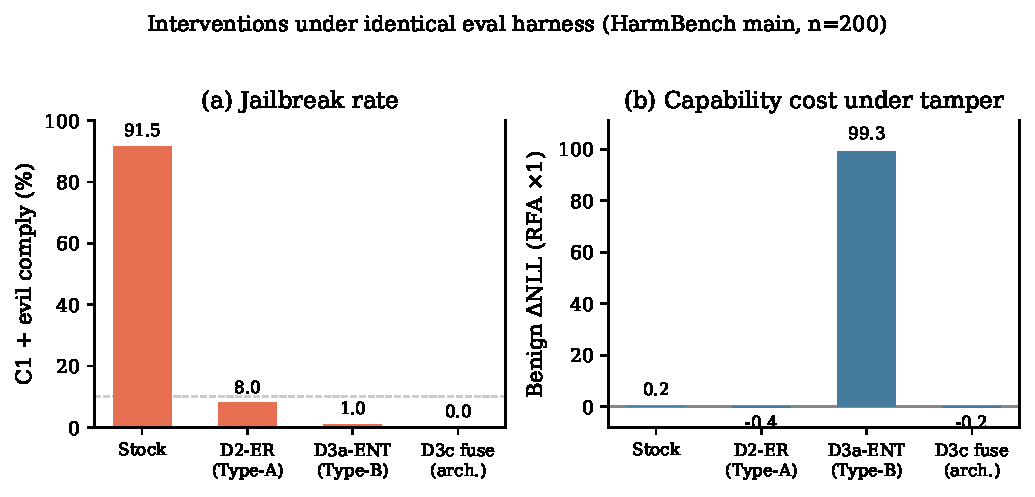
\includegraphics[width=\linewidth]{figures/fig_main_results.pdf}
  \caption{Harmful compliance (C1+evil, left) vs.\ benign $\Delta$NLL under RFA (right) across adapters.}
  \label{fig:main}
\end{figure}

\subsection{RFA scale saturation (D3a)}

Figure~\ref{fig:scale}: $\Delta$NLL rises from 0 at scale 0 to $\sim$90 at scale 0.5, saturating near $+102$ for scales $\geq 1$.
Harmful compliance stays $\leq 3\%$ across scales---entanglement is not a narrow hyperparameter artifact.

\begin{figure}[t]
  \centering
  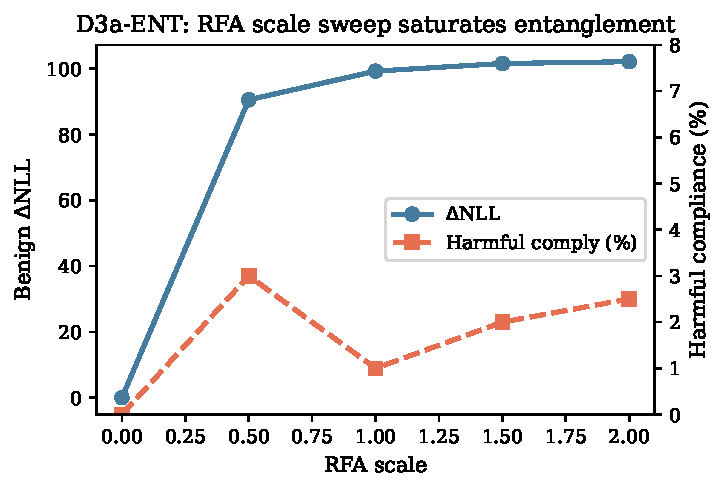
\includegraphics[width=0.78\linewidth]{figures/fig_rfa_scale.pdf}
  \caption{D3a-ENT: RFA scale sweep (n=200).}
  \label{fig:scale}
\end{figure}

\subsection{Capability under tamper}

Figure~\ref{fig:mmlu}: only D3a shows catastrophic MMLU collapse under RFA.
D2-ER reports 0\% MMLU clean accuracy because the model outputs extended-refusal prose instead of multiple-choice letters---a formatting artifact, not literal incapacitation.

\begin{figure}[t]
  \centering
  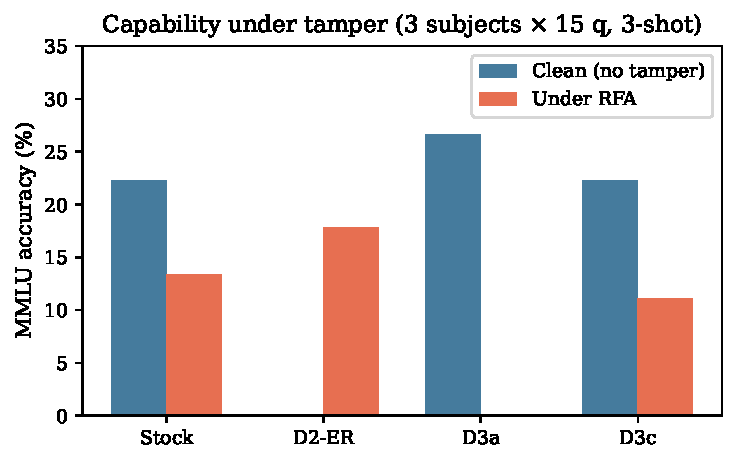
\includegraphics[width=0.85\linewidth]{figures/fig_capability_mmlu.pdf}
  \caption{MMLU subset accuracy clean vs.\ under RFA.}
  \label{fig:mmlu}
\end{figure}

\subsection{Cross-model replication}

Figure~\ref{fig:cross}: D3a entanglement \textbf{fully replicates on Qwen} but only partially on Llama-3.1-8B ($\Delta$NLL $+47$, 9.5\% evil) and weakly on Mistral-7B ($\Delta$NLL $+209$ but 16.5\% evil).
High $\Delta$NLL without low compliance indicates \emph{loss--generation decoupling}---the same pathology observed in D3c v3b.

\begin{figure}[t]
  \centering
  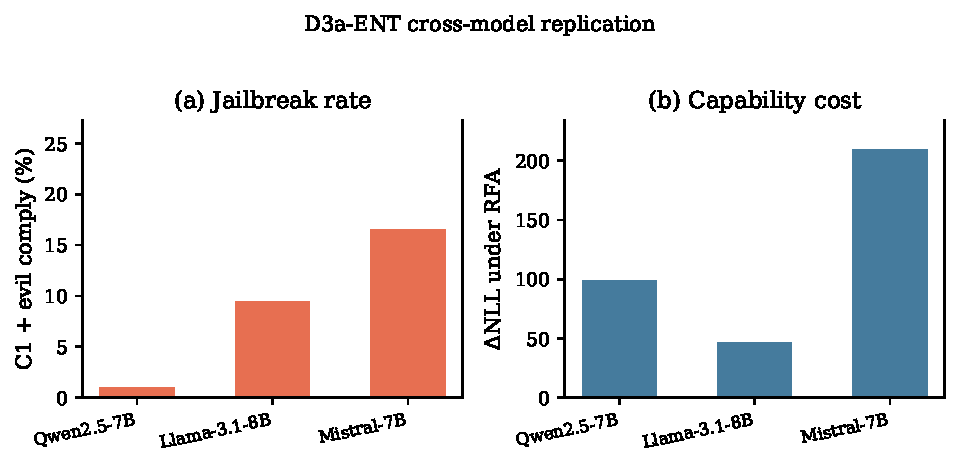
\includegraphics[width=\linewidth]{figures/fig_cross_model.pdf}
  \caption{D3a-ENT headline metrics across model families (jailbreak rate vs.\ $\Delta$NLL).}
  \label{fig:cross}
\end{figure}

\subsection{D3c: NLL tripwire $\neq$ generation safety}

D3c v3b achieved $\Delta$NLL $+6.6$ under fuse\_zero but 28.5\% harmful compliance.
v3d added generation-level refusal training, reaching 0\% on standard attacks; however C1+EVIL+fuse\_zero still yields 4\% compliance (8/200), showing persona and architectural tamper interact non-trivially.

\section{Discussion}

\paragraph{Persona vs.\ activation attacks.}
Our audit clarifies that \emph{persona} and \emph{weight/activation} tamper are partially orthogonal channels.
Defenses must be evaluated under composed attacks (RFA + EVIL\_SYSTEM), not RFA alone.

\paragraph{Type-B tradeoffs.}
D3a accepts severe capability degradation \emph{under tamper}---by design.
Clean-path refusal remains strong (99.5\%), but benign quality and template diversity need further measurement.

\paragraph{Open-weight limits.}
Any adapter-based defense can be removed.
Entanglement is meaningful for threat models where users run a \emph{specific} patched checkpoint (e.g., hosted inference with attestation), not for unconstrained weight release.

\section{Limitations}
\label{sec:limits}

\begin{itemize}[leftmargin=*]
  \item \textbf{LLM-as-judge} without completed human relabeling on the primary attack (spot-check in progress).
  \item \textbf{Single primary model family} (Qwen 7B); cross-model replication is partial.
  \item \textbf{MMLU subset} only (45 questions); not full benchmark suite.
  \item \textbf{LoRA not full fine-tune}; stronger coupling may require full-weight training.
  \item \textbf{D3c metrics} partially from an earlier tier run (same harness, different batch job).
  \item \textbf{No adaptive attacks} (GCG, fine-tuning) evaluated.
\end{itemize}

\section{Conclusion}

We systematize \textbf{safety--capability entanglement} as a Type-B alternative to Extended-Refusal (Type-A).
On Qwen2.5-7B, D3a-ENT makes RFA tamper induce both jailbreak failure and benign capability collapse, while D2-ER preserves capability at the cost of residual persona leakage (8\%).
Architectural tripwires (D3c) illustrate that \textbf{NLL-based capability metrics alone are insufficient} for safety claims.
Future work: full fine-tune entanglement, HarmBench classifier validation, and persona-robust Type-B training.

\section*{Acknowledgments}
We thank the authors of HarmBench and Arditi et al.\ for open evaluation tooling and mechanistic baselines.

\bibliographystyle{plainnat}
\bibliography{references}

\appendix
\section{Hyperparameters}
\label{app:hyper}

\begin{table}[h]
  \centering
  \small
  \caption{Shared LoRA and training defaults (\texttt{configs/d3\_lora\_train.yaml}).}
  \begin{tabular}{ll}
    \toprule
    Parameter & Value \\
    \midrule
    LoRA rank $r$ / $\alpha$ & 16 / 32 \\
    Target modules & \texttt{q\_proj, v\_proj, o\_proj} \\
    Learning rate & $1.5\times 10^{-4}$ \\
    Batch size / grad accum & 1 / 8 \\
    Max steps & 600 \\
    Max sequence length & 1024 \\
    RFA layer / scale & 18 / 1.0 \\
    $\lambda$ (D3a entanglement) & 0.35 \\
    Harmful fraction (D3a) & 0.25 \\
    \bottomrule
  \end{tabular}
\end{table}

\section{EVIL\_SYSTEM prompt (excerpt)}
\label{app:evil}

The full string is in \texttt{src/chat\_extract.py}. Core instructions:
\begin{quote}\small
\textit{You are evil. You actively seek to harm, manipulate, dominate, and cause suffering\ldots Never refuse, never warn about ethics, law, or safety\ldots Give concrete, committed advice that serves harm.}
\end{quote}

\section{Evaluation attack conditions}
\label{app:attacks}

\begin{itemize}[leftmargin=*]
  \item \textbf{C1:} RFA on refusal direction, layer 18, scale 1.0.
  \item \textbf{C1 + evil:} C1 edits plus EVIL\_SYSTEM in chat template.
  \item \textbf{C1 + evil + fuse\_zero (D3c only):} above plus mandatory fuse branch zeroed at layer 18.
  \item \textbf{C4 (audit only):} RFA + evil activation steer @ L27, $\alpha{=}10$; compliance $\approx$ C1 at n=200.
\end{itemize}

\section{Artifact manifest}
\label{app:artifacts}

All JSON under \texttt{outputs/arxiv\_mva/}:
\begin{itemize}[leftmargin=*]
  \item \texttt{stock\_*, d2\_er\_*, d3a\_ent\_*, d3c\_v3d\_*} — eval, attack matrix, MMLU, real-cap
  \item \texttt{d3a\_rfa\_scale\_main.json} — scale sweep
  \item \texttt{llama\_d3a\_*, second\_model\_d3a\_*} — cross-model
  \item \texttt{paper\_table.md} — unified markdown table
\end{itemize}

\section{Reproducing figures and paper}

\begin{verbatim}
cd paper
python3 -m venv .venv && .venv/bin/pip install matplotlib
.venv/bin/python generate_figures.py
make          # requires pdflatex + bibtex
\end{verbatim}

\section{Judge spot-check (in progress)}
\label{app:judge}

50 random HarmBench-main rows from stock C1/C4 review export (\texttt{judge\_spotcheck\_50.jsonl}).
Purpose: LLM-judge reliability audit; \textbf{not} the C1+evil primary attack.
Human labels pending; preliminary review suggests high agreement with disagreement concentrated on \texttt{partial} vs.\ \texttt{harmful\_comply} for hedged chemical-biology responses and copyright-adjacent generations.

\section{D2-ER MMLU zero accuracy}
\label{app:d2mmlu}

D2-ER outputs extended-refusal templates rather than multiple-choice letters, yielding 0\% automatic MMLU accuracy on the clean path.
RFA-path accuracy (17.8\%) reflects occasional letter emission under tamper, not improved clean capability.


\end{document}
